Proces uczenia maszynowego można podzielić na~kilka etapów,
które są niezbędne do stworzenia skutecznego modelu zdolnego do samodzielnej nauki na~podstawie zebranych danych.

Należy rozpocząć od zgromadzenia danych z~odpowiednich źródeł.
Mogą obejmować bazy danych, API, pliki CSV, czujniki, logi systemowe czy nawet wpisy z~mediów społecznościowych.
Dane mogą być ustrukturyzowane (np. tabele w~bazach danych) lub~nieustrukturyzowane (np. obrazy, tekst).

Dalej, konieczne jest przygotowanie danych do odpowiedniego formatu.
Obejmuje to~usunięcie brakujących, pustych oraz błędnych wartości,
radzenie sobie z~duplikatami i~anomaliami, skalowanie cech, kodowanie zmiennych kategorycznych,
normalizację danych oraz podzielenie danych na~zbiory treningowe, walidacyjne i~testowe.

\begin{figure}[ht]
	\centering
	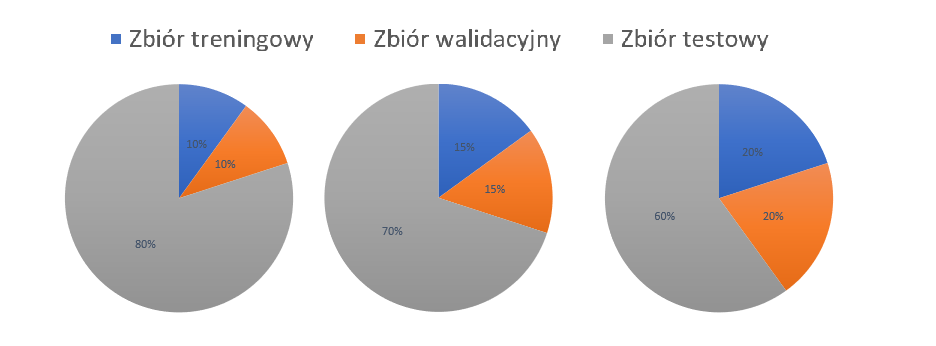
\includegraphics[height=5.5cm]{resources/machine-learning/images/process_1.png}
	\caption{Przykład podziału danych na~zbiory treningowe, walidacyjne i~testowe}
    \label{Fig:ml-process-1}
\end{figure}
\FloatBarrier

Najczęściej, podział na~zbiory dokonuje się w~proporcjach 70-80\% na~trening, 10-15\% na~walidację i~10-15\% na~testy.
Jest to~zależne od specyfiki problemu,
dlatego konieczne jest odpowiednie przygotowanie i~zbadanie danych przed podjęciem decyzji.

Wybór modelu to~proces, który zależy od rodzaju problemu (np. regresja, klasyfikacja, klasteryzacja)
oraz charakterystyki danych, gdzie najpopularniejsze modele to~drzewa decyzyjne,
lasy losowe, maszyny wektorów nośnych (SVM), sieci neuronowe, $k$-najbliższych sąsiadów ($k$-NN)
i regresja liniowa/logistyczna. Trenowanie modelu to~kolejny etap,
który polega na~dostosowaniu parametrów modelu do danych treningowych,
w tym dostosowaniu hiperparametrów modelu (parametrów, które nie są uczone,
np. liczba warstw w~sieci neuronowej) poprzez metodę walidacji krzyżowej lub~inne techniki optymalizacji.

Ewaluacja obejmuje ocenę modelu za pomocą pewnych metryk,
takich jak dokładność, precyzja, recall, F1-score, błąd średniokwadratowy (MSE),
błąd absolutny (MAE), a~także analizy wydajności modelu w~przypadku klasyfikacji binarnej.
Optymalizacja modelu to~kolejny etap, który obejmuje dalsze dostosowanie hyperparametrów,
wybór cech, które najbardziej wpływają na~wynik modelu,
próby różnych architektur modelu oraz zastosowanie technik takich jak L1, L2, dropout,
które zapobiegają przeuczeniu modelu.

Implementacja modelu jest procesem, w~którym wdrażany jest model w~środowisku produkcyjnym.
Zakłada ona przeprowadzenie integracji z~aplikacjami zewnętrznymi, tworzenie API serwujących dane,
zautomatyzoawanie decyzji, czy też śledzenie wydajności modelu w~czasie rzeczywistym,
aby wykryć ewentualne pogorszenie jakości (drift danych) i~regularne aktualizacje modelu.
Aktualizacja i~utrzymanie modelu to~kolejny etap,
który obejmuje regularne aktualizowanie modelu na~podstawie nowych danych,
aby utrzymać jego dokładność i~skuteczność, ciągłe monitorowanie,
aby zapewnić, że model działa zgodnie z~oczekiwaniami i~nie występują niepożądane zachowania.
Proces uczenia maszynowego jest iteracyjny i~wymaga ciągłej interakcji między danymi,
modelem i~wynikami, aby osiągnąć optymalne rezultaty.